\documentclass{article}
\usepackage{graphicx}
\usepackage[utf8]{inputenc}
\usepackage[cyr]{aeguill}
\usepackage{xspace}
\usepackage{amsmath}
\usepackage[english,francais]{babel}
\usepackage{url}
\usepackage{hyperref}
\let\urlorig\url
\renewcommand{\url}[1]{%
  \begin{otherlanguage}{english}\urlorig{#1}\end{otherlanguage}%
}
\renewcommand{\contentsname}{Sommaire} % si tableofcontents au début
\newcommand{\Numero}{\No}
\newcommand{\numero}{\no}
%\newcommand{\fup}[1]{\up{#1}}
%%% N'oubliez pas les espaces devant les doubles ponctuations
\NoAutoSpaceBeforeFDP

\title{Rapport CR12:\\
Reconnaissance de locuteur}
\author{Antoine Plet\\
Thomas Sibut-Pinote}
\date{Janvier 2014}

\begin{document}

\maketitle

\section{Introduction}
Le but de ce projet était d'implémenter un programme de reconnaissance de locuteur, c'est-à-dire, à partir de données d'entraînement, d'identifier si une personne qui parle est l'un des sujets entraînés ou non.

Nous avons essayé de retrouver les résultats du papier "Kernel Based Text-Independent Speaker Verification" de Mariéthoz, Grandvalet et Bengio.

Nous avons commencé par coder un svm(\ref{svm}).

Puis nous avons codé le kernel perceptron pour pouvoir tester plusieurs noyaux, l'objectif (atteint(?) A CHANGER QUAND ON SAURA) étant d'arriver au noyau de Fisher(\ref{fisher}).

Nous avons enfin fait diverses validations (\ref{validation}) sur des données générées (\ref{donnees}) par nous-mêmes.

\section{Particularités d'implémentation}
\label{implémentation}
Nous avons travaillé sur un dépôt github (\url{https://github.com/tomsib2001/speaker-recognition}).

Nous avons utilisé le langage Python qui nous était le plus familier. Cependant, la très utile bibliothèque Voicebox étant écrite en Matlab/Octave, nous avons dû interfacer Python avec Octave (\texttt{octaveIO.py}).

%% parler ici des graphes en GNUplot s'ils existent...

\section{Répartition du travail}
\label{répartition}
\subsection{Antoine}
\subsection{Thomas}
\subsection{Ensemble}

\section{Choix des données}
Nous avons pu disposer de 5 enregistrements de personnes lisant tous la même série de 12 phrases.

Nous nous sommes de plus enregistrés tous les deux.

Enfin, nous avons pris un enregistrement d'une personnalité politique ainsi que celui d'un imitateur, pour voir à quel point il arrivait à se faire passer pour le premier. Les résultats sont en \ref{imitateur}.
\section{Représentation des données}
\label{representation}
Conformément à ce que propose l'article, nous avons choisi de transformer les données en extrayant des caractéristiques discriminantes, dont les premières sont des coefficients d'une transformée discrète de cosinus (DCT), et les suivantes sont leur dérivée puis diverses fonctions du signal.

Pour cela, nous avons utilisé la librairie Voicebox (\url{http://www.ee.ic.ac.uk/hp/staff/dmb/voicebox/voicebox.html}).
\section{SVM}
\label{svm}
\subsection{SGD}
\label{sgd}
Nous avons commencé par programmer utilisant la technique de la Descente de Gradient Stochastique en considérant le problème:

\begin{equation}
\label{eq:primalSVM}
  \left\{
    \begin{array} {lll}
      \displaystyle\min_{w,b,\xi_i} & \frac{1}{2} \|w\|^2 + C\displaystyle\sum\limits_{i=1}^{n}\xi_i&\\
      \mbox{avec} &y_i(w^\top  x_i+b) \geq 1 - \xi_i,\quad & i=1,\dots ,n  \\
      \mbox{et} &\xi_i \geq 0 , &i=1,\dots ,n  \\
    \end{array}
  \right.
\end{equation}

On va appliquer la technique de la descente stochastique de gradient vue en cours, à la fonction convexe
\[ f_{obj}(w) := \frac{1}{2} \|w\|^2 + C\displaystyle\sum\limits_{i=1}^{n}l_i(w) \]
où $l_i(w) = \max (0, 1 - y_i (w \cdot x_i + b)) = \mathrm{hinge}(y_i (w \cdot x_i + b))$ est la fonction de coût.
On calcule un subgradient de $\mathrm{hinge}(x) = max(0,1-x)$:
\[ \partial \mathrm{hinge}(x)(h) = \begin{cases} 0 &\mbox{si } x>1 \\
-\frac{h}{2} & \mbox{si } x=1\\
-h & \mbox{si } x<1\\
 \end{cases}\]
 
 soit 
\[ \nabla \mathrm{hinge}(x) = \begin{cases} 0 &\mbox{si } x>1 \\
-\frac{1}{2} & \mbox{si } x=1\\
-1 & \mbox{si } x<1\\
 \end{cases}\]
On écrit en fait $f_{obj}$ comme une fonction de $\tilde{w} = (w,b)$ (car $b$ est un paramètre à trouver).
On a $l_i (\tilde{w}) = max(0, 1 - y_i \langle \tilde{w} , (x,1) \rangle)$ de sorte que
\[ \nabla l_i(\tilde{w}) = \begin{cases} 0 &\mbox{si } \langle \tilde{w}, (x,1) \rangle >1 \\
-\frac{y_i}{2} (x,1) & \mbox{si } \langle \tilde{w}, (x,1) \rangle=1\\
-y_i (x,1) & \mbox{si } \langle \tilde{w}, (x,1) \rangle<1\\
 \end{cases}\]
 et enfin
 \[ \nabla f_{obj}(w,b) = w + C \cdot \displaystyle\sum\limits_{i=1}^{n} \nabla l_i(\tilde{w}). \]

\subsubsection{Premiers Tests}
\label{donnees}
Afin de tester "visuellement" notre implémentation\footnote{\texttt{sgd.py}} en Python, nous avons écrit un générateur de données en dimension 2 qui fabrique des points répartis selon deux lois de moyennes différentes $\mu_1$ et $\mu_2$ uniformes respectivement sur $\lbrack \mu_1 - 1, \mu_1 + 1\rbrack$ et $\lbrack \mu_2 - 1, \mu_2 + 1\rbrack$.
Nous avons ensuite écrit une fonction qui affiche les points ainsi que la solution trouvée par la descente stochastique.

\begin{figure}[!h]
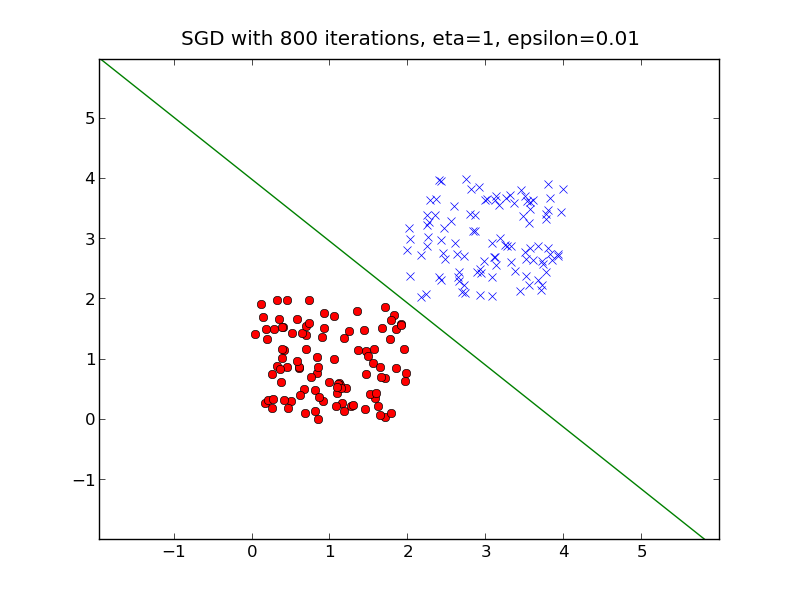
\includegraphics[width=0.85\textwidth]{../SGD}
\end{figure}


\section{Kernel Perceptron}
\label{kernelperceptron}
En vue de tester différents noyaux mentionnés par l'article, nous avons implémenté l'algorithme du Kernel Perceptron\footnote{\texttt{kernel\_perceptron.py}}.

\subsection{Premiers tests}
Comme pour la SGD, nous avons testé le Kernel Perceptron sur des données générées avec le noyau trivial qui correspond à rester dans l'espace ambiant avec son produit scalaire) en dimension 2:

IMAGE GÉNÉRÉE PAR ANTOINE A INSERER ICI


\section{Noyau Gaussien}
\label{gaussien}
\section{Noyau de Fisher}
\label{fisher}
\subsection{GMM}
Le noyau de Fisher est construit à partir de modèles générateurs, dans notre cas, un GMM\footnote{Gaussian Mixture Model}.
Celui-ci produit à partir des données d'entraînement des paramètres $\theta_0 = \lbrace \mu_m^0, \sigma_m, \pi_m \rbrace_{m=1}^M$ décrivant $M$ gaussiennes\footnote{C'est-à-dire plus précisément de vecteurs gaussiens, dans le cas général où les données sont en dimension $k$.} de moyenne $\mu_m$ et de variance $\sigma_m$, et qui sont une approximation de la distribution des données.

Dans notre cas, on réalise un GMM pour un $M$ fixé (à partir de tests empiriques) sur des paquets de $T$ \og frames \fg \footnote{On rappelle qu'une frame représente une fenêtre de 20ms.}.

Pour cela, nous avons d'abord utilisé la librairie \texttt{gaussmix} de Voicebox avant de passer à la fonction mixture de \texttt{Scikit-Learn} pour Python à cause de problèmes de terminaison.
\subsection{Noyau de Fisher}
Étant donné un échantillon $\bar{x}$, le vecteur des scores de Fisher est:
\[u_{\bar{x}} = \nabla_{\theta} \log p (\bar{x} | \theta) \]

Alors le Kernel de Fisher est défini par:
\[K(\bar{x}_i,\bar{x}_j) = u_{\bar{x}_i}^{T} I(\theta)^{-1} u_{\bar{x}_j}\]
où $I(\theta)$ est la matrice d'information de Fisher, dont l'article affirme qu'on peut sans grande perte l'approximer par l'identité pour cette application. Nous ferons donc cette hypothèse et ne parlerons plus de cette matrice.

(EXPLICATIONS INTERMEDIAIRES)

Finalement, on a:
\[ K(\bar{x}_i,\bar{x}_j) = \sum_{m=1}^M (n_{i,m} \Sigma_m^{-2} (\mu_m^i - \mu_m^0))^{T} (n_{j,m} \Sigma_m^{-2} (\mu_m^j - \mu_m^0)) \]
avec
\[n_{i,m} = \sum_{t=1}^{T} P(m | x_i^t),\]
$x_i^t$ étant la $t$-ième frame de $x_i$, $P(m | x_i^t)$ mesurant le taux d'appartenance de $x_i^t$ à la $m$-ième gaussienne, donnée qui est fournie par le GMM.


\section{Validation}
\label{validation}
\subsection{Validation croisée}
Pour choisir la constante $C$ la plus adaptée à un ensemble d'entraînement pour la technique de la SGD (\ref{sgd}), nous avons utilisé le protocole suivant:
\begin{itemize}
\item On choisit un sous-ensemble $S$ des locuteurs enregistrés.
\item Pour chaque locuteur, on partage les données selon les ratios suivants:
\begin{itemize}
\item $r_1$ vont dans l'ensemble d'entraînement;
\item $r_2$ vont dans l'ensemble de validation;
\item $1 - r_1 - r_2$ vont dans l'ensemble de \og post-validation \fg, accompagnés des locuteurs que l'on avait exclus à la première étape.
\end{itemize}
\item Pour chaque $C$ dans $2^{-k}, \dotsi, 1, \dotsi 2^k$, on calcule un $w$ correspondant à la valeur de $C$, et on calcule le taux de réussite sur l'ensemble de validation.
\item On en déduit une meilleure valeur de $C$, que l'on teste sur le troisième ensemble de \og post-validation \fg. Cela permet entre autres de voir si le résultat trouvé résiste aux \og attaques \fg, c'est-à-dire des locuteurs qui n'ont jamais été vus ni traités.
\end{itemize}

\begin{figure}[!h]
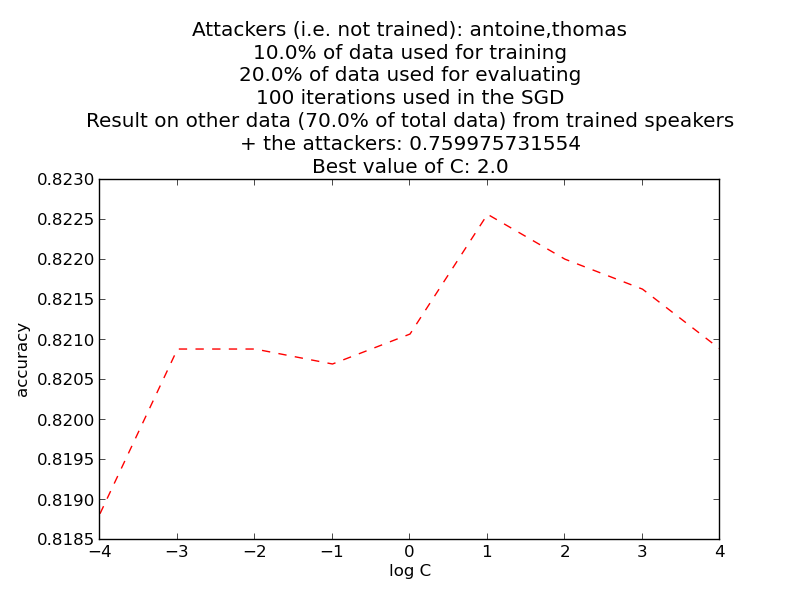
\includegraphics[width=0.85\textwidth]{../bestC}
\end{figure}
Cela donne par exemple la courbe ci-dessus, pour $k=4$ et les autres paramètres donnés sur le graphique:

On obtient $75.99 \%$ de réussite sur le troisième ensemble qui contient, en plus de données des locuteurs déjà entraînés, deux \og attaquants \fg. Ici, la meilleure valeur de $C$ est $2^1 = 2$.
\section{Résultats}
\subsection{Imitateur}
\label{imitateur}
\end{document}